% A LaTeX (non-official) template for ISAE projects reports
% Copyright (C) 2014 Damien Roque
% Version: 0.2
% Author: Damien Roque <damien.roque_AT_isae.fr>

\documentclass[a4paper,12pt]{book}
\usepackage[utf8]{inputenc}
\usepackage[T1]{fontenc}
\usepackage[french]{babel} % If you write in French
%\usepackage[english]{babel} % If you write in English
\usepackage{a4wide}
\usepackage{graphicx}
\graphicspath{{images/}}
\usepackage{subfig}
\usepackage{tikz}
\usetikzlibrary{shapes,arrows}
\usepackage{pgfplots}
\pgfplotsset{compat=newest}
\pgfplotsset{plot coordinates/math parser=false}
\newlength\figureheight
\newlength\figurewidth
\pgfkeys{/pgf/number format/.cd,
set decimal separator={,\!},
1000 sep={\,},
}
\usepackage{ifthen}
\usepackage{ifpdf}
\ifpdf
\usepackage[pdftex]{hyperref}
\else
\usepackage{hyperref}
\fi
\usepackage{color}
\hypersetup{%
colorlinks=true,
linkcolor=black,
citecolor=black,
urlcolor=black}

\renewcommand{\baselinestretch}{1.05}
\usepackage{fancyhdr}
\pagestyle{fancy}
\fancyfoot{}
\fancyhead[LE,RO]{\bfseries\thepage}
\fancyhead[RE]{\bfseries\nouppercase{\leftmark}}
\fancyhead[LO]{\bfseries\nouppercase{\rightmark}}
\setlength{\headheight}{15pt}

\let\headruleORIG\headrule
\renewcommand{\headrule}{\color{black} \headruleORIG}
\renewcommand{\headrulewidth}{1.0pt}
\usepackage{colortbl}
\arrayrulecolor{black}

\fancypagestyle{plain}{
  \fancyhead{}
  \fancyfoot[C]{\thepage}
  \renewcommand{\headrulewidth}{0pt}
}

\makeatletter
\def\@textbottom{\vskip \z@ \@plus 1pt}
\let\@texttop\relax
\makeatother

\makeatletter
\def\cleardoublepage{\clearpage\if@twoside \ifodd\c@page\else%
  \hbox{}%
  \thispagestyle{empty}%
  \newpage%
  \if@twocolumn\hbox{}\newpage\fi\fi\fi}
\makeatother

\usepackage{amsthm}
\usepackage{amssymb,amsmath,bbm}
\usepackage{array}
\usepackage{bm}
\usepackage{multirow}
\usepackage[footnote]{acronym}

\newcommand*{\SET}[1]  {\ensuremath{\mathbf{#1}}}
\newcommand*{\VEC}[1]  {\ensuremath{\boldsymbol{#1}}}
\newcommand*{\FAM}[1]  {\ensuremath{\boldsymbol{#1}}}
\newcommand*{\MAT}[1]  {\ensuremath{\boldsymbol{#1}}}
\newcommand*{\OP}[1]  {\ensuremath{\mathrm{#1}}}
\newcommand*{\NORM}[1]  {\ensuremath{\left\|#1\right\|}}
\newcommand*{\DPR}[2]  {\ensuremath{\left \langle #1,#2 \right \rangle}}
\newcommand*{\calbf}[1]  {\ensuremath{\boldsymbol{\mathcal{#1}}}}
\newcommand*{\shift}[1]  {\ensuremath{\boldsymbol{#1}}}

\newcommand{\eqdef}{\stackrel{\mathrm{def}}{=}}
\newcommand{\argmax}{\operatornamewithlimits{argmax}}
\newcommand{\argmin}{\operatornamewithlimits{argmin}}
\newcommand{\ud}{\, \mathrm{d}}
\newcommand{\vect}{\text{Vect}}
\newcommand{\sinc}{\ensuremath{\mathrm{sinc}}}
\newcommand{\esp}{\ensuremath{\mathbb{E}}}
\newcommand{\hilbert}{\ensuremath{\mathcal{H}}}
\newcommand{\fourier}{\ensuremath{\mathcal{F}}}
\newcommand{\sgn}{\text{sgn}}
\newcommand{\intTT}{\int_{-T}^{T}}
\newcommand{\intT}{\int_{-\frac{T}{2}}^{\frac{T}{2}}}
\newcommand{\intinf}{\int_{-\infty}^{+\infty}}
\newcommand{\Sh}{\ensuremath{\boldsymbol{S}}}
\newcommand{\C}{\SET{C}}
\newcommand{\R}{\SET{R}}
\newcommand{\Z}{\SET{Z}}
\newcommand{\N}{\SET{N}}
\newcommand{\K}{\SET{K}}
\newcommand{\reel}{\mathcal{R}}
\newcommand{\imag}{\mathcal{I}}
\newcommand{\cmnr}{c_{m,n}^\reel}
\newcommand{\cmni}{c_{m,n}^\imag}
\newcommand{\cnr}{c_{n}^\reel}
\newcommand{\cni}{c_{n}^\imag}
\newcommand{\tproto}{g}
\newcommand{\rproto}{\check{g}}
\newcommand{\LR}{\mathcal{L}_2(\SET{R})}
\newcommand{\LZ}{\ell_2(\SET{Z})}
\newcommand{\LZI}[1]{\ell_2(\SET{#1})}
\newcommand{\LZZ}{\ell_2(\SET{Z}^2)}
\newcommand{\diag}{\operatorname{diag}}
\newcommand{\noise}{z}
\newcommand{\Noise}{Z}
\newcommand{\filtnoise}{\zeta}
\newcommand{\tp}{g}
\newcommand{\rp}{\check{g}}
\newcommand{\TP}{G}
\newcommand{\RP}{\check{G}}
\newcommand{\dmin}{d_{\mathrm{min}}}
\newcommand{\Dmin}{D_{\mathrm{min}}}
\newcommand{\Image}{\ensuremath{\text{Im}}}
\newcommand{\Span}{\ensuremath{\text{Span}}}

\newtheoremstyle{break}
  {11pt}{11pt}%
  {\itshape}{}%
  {\bfseries}{}%
  {\newline}{}%
\theoremstyle{break}

%\theoremstyle{definition}
\newtheorem{definition}{Définition}[chapter]

%\theoremstyle{definition}
\newtheorem{theoreme}{Théorème}[chapter]

%\theoremstyle{remark}
\newtheorem{remarque}{Remarque}[chapter]

%\theoremstyle{plain}
\newtheorem{propriete}{Propriété}[chapter]
\newtheorem{exemple}{Exemple}[chapter]

\parskip=5pt
%\sloppy

\begin{document}

%%%%%%%%%%%%%%%%%%
%%% First page %%%
%%%%%%%%%%%%%%%%%%

\begin{titlepage}
\begin{center}


\includegraphics[width=0.6\textwidth]{logo-isae-supaero}\\[1cm]

{\large SXS}\\[0.5cm]

{\large Projet Ingénierie et Entreprise}\\[0.5cm]

% Title
\rule{\linewidth}{0.5mm} \\[0.4cm]
{ \huge \bfseries Machine Learning pour la valorisation de données vol ADS-B \\[0.4cm] }
\rule{\linewidth}{0.5mm} \\[1.5cm]

% Author and supervisor
\noindent
\begin{minipage}{0.4\textwidth}
  \begin{flushleft} \large
    \emph{Auteurs :}\\
    Alexis \textsc{Vandewalle}\\
    Naihao \textsc{Liu}\\
    Ziqing \textsc{Wu}\\
    Loïc \textsc{Tiberghien}\\
    Baptiste \textsc{Gaudron-Desjardins}\\
    Zhengyu \textsc{Jiang}
    
  \end{flushleft}
\end{minipage}%
\begin{minipage}{0.4\textwidth}
  \begin{flushright} \large
    \emph{Encadrants :} \\
    Nicolas \textsc{Canouet}\\
    Matthieu \textsc{Bessac}
  \end{flushright}
\end{minipage}

\vfill

% Bottom of the page
{\large Version 0.1 du\\ \today}

\end{center}
\end{titlepage}

%%%%%%%%%%%%%%%%%%%%%%%%%%%%%
%%% Non-significant pages %%%
%%%%%%%%%%%%%%%%%%%%%%%%%%%%%

\frontmatter


\clearpage
\tableofcontents


%%%%%%%%%%%%%%%%%%%%%%%%%%%%%%%%%%%%%%%%%%%%
%%% Content of the report and references %%%
%%%%%%%%%%%%%%%%%%%%%%%%%%%%%%%%%%%%%%%%%%%%

\mainmatter
\pagestyle{fancy}

\cleardoublepage

\chapter*{Description du projet}
\addcontentsline{toc}{chapter}{Description du projet}
\label{chap:description}
%\minitoc
L'entreprise Liebherr commercialise des systèmes d'air conditionné qui équipent
la totalité des avions de la gamme A320. Elle assure également la maintenance de ces systèmes sur ces avions. Afin d'être plus compétitive, elle souhaite améliorer son service de maintenance. La firme a constaté que plusieurs de ses clients rencontrent des problèmes et supposent que ceux-ci proviennent de leur manière d'utiliser leurs avions.

Le but de notre projet est d'établir une classification des compagnies aériennes par modes d'opération. Les modes d'opération ont un impact important sur le design des systèmes d'air commercialisés par la société et peuvent expliquer les problèmes rencontrés en service par les compagnies aériennes.

Afin de réaliser cette classification, nous souhaitons exploiter les données de vol ADS-B. L'automatic dependent surveillance-broadcast(ADS-B) est un système de surveillance coopératif pour le contrôle du traffic aérien. Les avions qui utilisent ce système envoient périodiquement leur position, vitesse de montée, vitesse de descente et altitude à des stations positionnées au sol. Les données sont disponibles sur des plateformes open source que l'on peut alors exploiter.

\section*{Objectifs}
\addcontentsline{toc}{section}{Objectifs}
Notre objectif principal sera d'établir une classification des compagnies aériennes par mode d'opération similaire. Cela implique:

\begin{itemize}
	\item extraire des données ADS-B les données de chaque avions de type A320
	\item calculer les phases de vol pour chaque vol
	\item trouver des descripteurs et les calculer pour chaque phase de vol
	\item réaliser une application web pour avoir un aperçu global des données calculées
	\item établir la classification final à partir des données calculées pour chaque vol
\end{itemize}

\section*{Parties prenantes}
\addcontentsline{toc}{section}{Parties prenantes}
Notre client est la société Liebherr avec notamment Nicolas Canouet qui est chargé de l'encadrement du projet. D'un point de vue gestion de projet, Matthieu Bessac se charge de nous accompagner.

\section*{Contraintes associées au projet}
\addcontentsline{toc}{section}{Contraintes associées au projet}
Notre projet se limite à l'étude des données produites par les avions de la gamme A320 puisque notre client ne cherche qu'à établir une classification pour ce type d'avion.

Pour le reste, la forme des rendus par le client est assez libre. Nous prévoyons donc de présenter nos résultats sous forme d'application web accompagnée d'un rapport.

\section*{Exigences}
\addcontentsline{toc}{section}{Exigences}
Les personnes impliquées dans le projet le sont pour une période courte et ne seront plus disponibles une fois le projet terminé. Nous nous devons donc de faire en sorte que nos rendus soient le plus claire possible afin que le client puissent exploiter nos résultats au mieux.

\section*{Synthèse}
\addcontentsline{toc}{section}{Synthèse}
Nous synthétisons dans cette partie le projet par un diagramme pieuvre qui relie les élément externes du système entre eux par l'intermédiaire de celui-ci.

\begin{figure}[!ht]
	\centering
	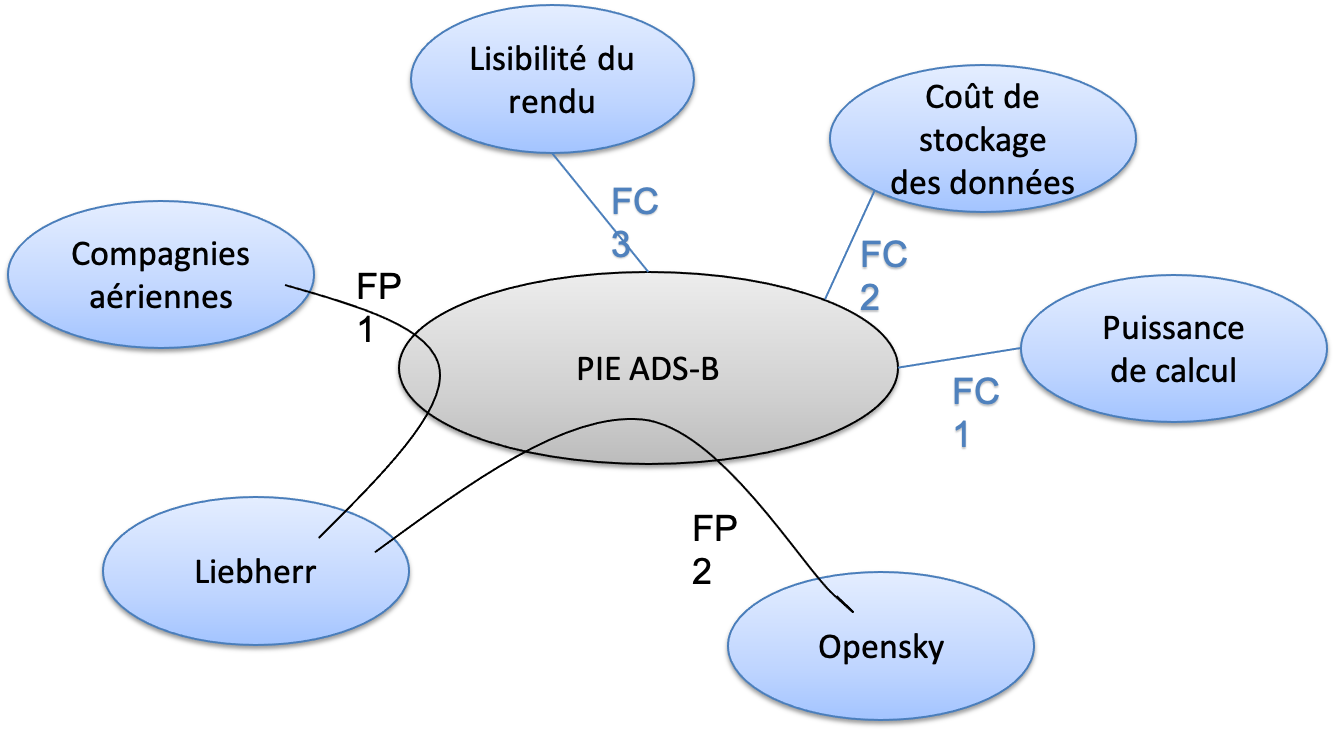
\includegraphics[width=15cm]{DiagrammePieuvre}
	\caption{
		Diagramme pieuvre du projet. FP1: classer les compagnies
		en fonction de leur mode d'opération, FP2: exploiter les données ADS-B
		, FC1: ne pas dépasser les ressources informatiques disponibles,
		FC2: respecter les coûts associés au stockage des données,
		FC3: rendre un projet exploitable par le client.
	}
	\label{fig:pieuvre}
\end{figure}

%%% Local Variables: 
%%% mode: latex
%%% TeX-master: "isae-report-template"
%%% End: 

\chapter*{Détails du projet}
\addcontentsline{toc}{chapter}{Détails du projet}
\markboth{Détails du projet}{Détails du projet}
\label{chap:detail}

Dans cette partie, nous présentons les grandes composantes de notre projet et nous explicitons plus en détail les livrables de notre projet.

\section*{Work Breakdown Structure}
\addcontentsline{toc}{section}{Work Breakdown Structure}
Le WBS suivant présente la décomposition de notre projet en plusieurs bloc que nous avons faite.

\begin{figure}[!h]
	\centering
	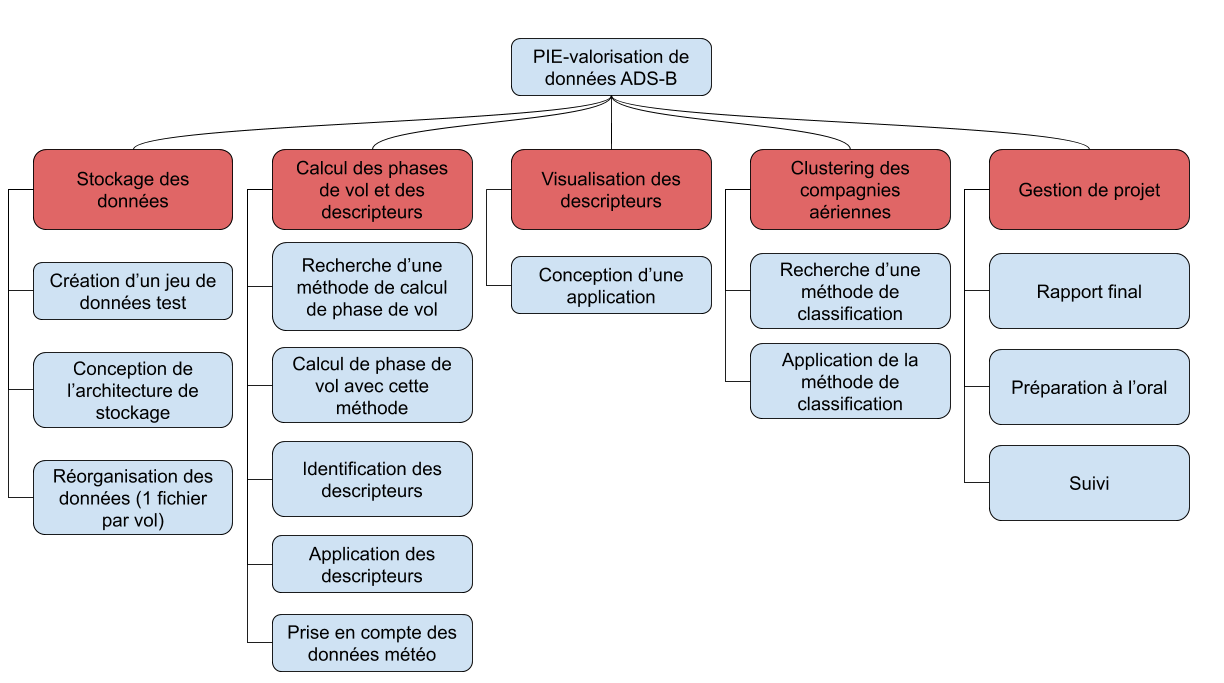
\includegraphics[width=12cm]{WBS}
	\caption{WBS}
	\label{fig:wbs}
\end{figure}
 
\section*{Livrables et critères d'acceptabilité}
\addcontentsline{toc}{section}{Livrables et critères d'acceptabilité}
Les livrables ainsi que leur critère d'acceptabilité sont présentés ci-dessous:
\begin{itemize}
	\item un plan de développement cohérent
	\item un compte-rendu répondant au problème initialement formulé par le client
	\item une soutenance PIE présentant le projet et son déroulement
	\item les codes sources commentés et facilement utilisable par le client
\end{itemize}

%%% Local Variables: 
%%% mode: latex
%%% TeX-master: "isae-report-template"
%%% End: 
\chapter*{Organisation du projet}
\addcontentsline{toc}{chapter}{Organisation du projet}
\label{sec:organisation}
\section*{Planning}
\addcontentsline{toc}{section}{Planning}
Les figures \ref{fig:mvp-plan}, \ref{fig:gestion-proj} et \ref{fig:r1-plan} montrent le planning que nous allons suivre pour réaliser notre projet.

\begin{figure}[!ht]
	\centering
	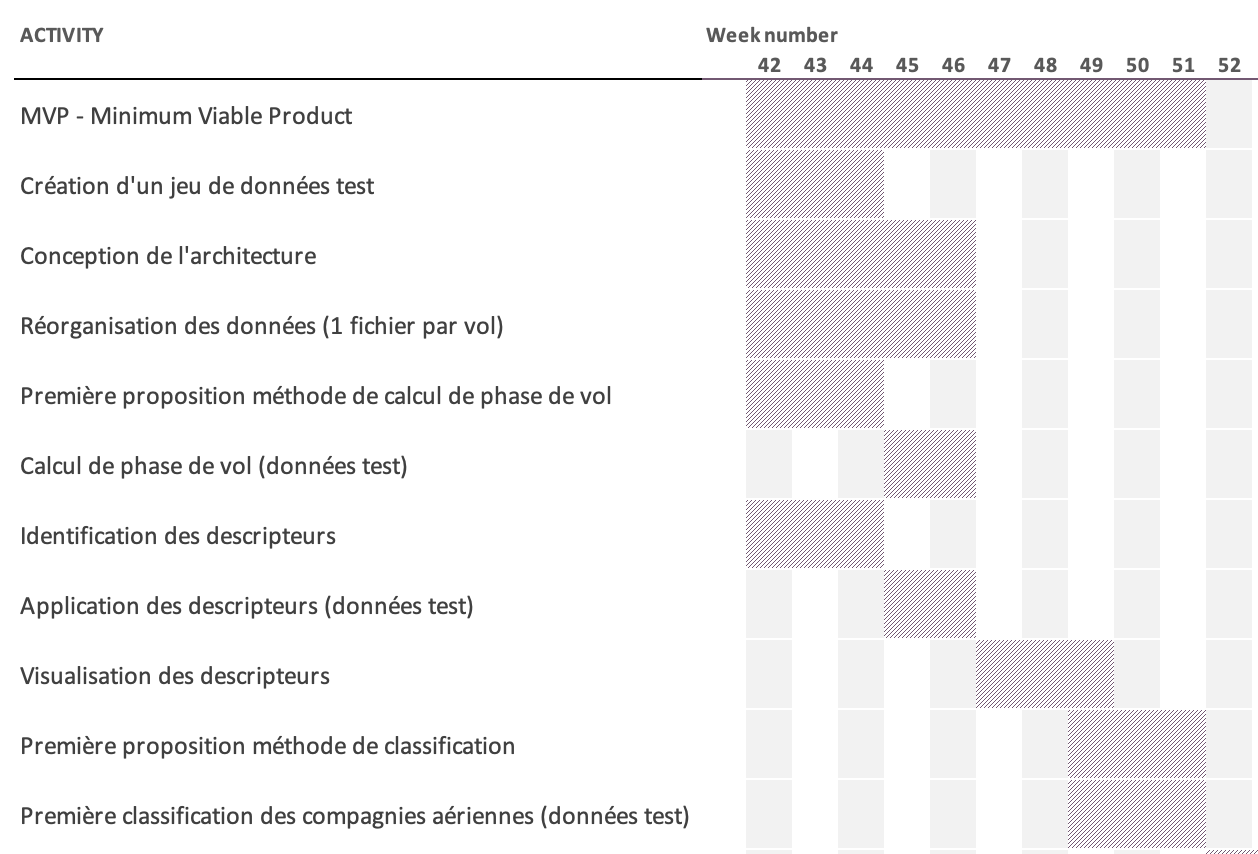
\includegraphics[width=15cm]{MVP planning}
	\caption{planning associé au produit minimal(MVP)}
	\label{fig:mvp-plan}
\end{figure}

\begin{figure}[!ht]
	\centering
	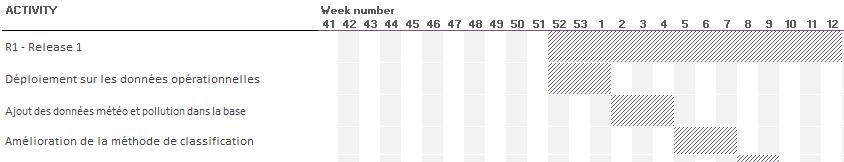
\includegraphics[width=15cm]{R1 planning}
	\caption{planning associé à la gestion de projet}
	\label{fig:r1-plan}
\end{figure}

\begin{figure}[!ht]
	\centering
	\includegraphics[width=15cm]{gestion projet}
	\caption{planning associé au produit minimal(MVP)}
	\label{fig:gestion-proj}
\end{figure}

\section*{Association des taches aux membres du projet}
\addcontentsline{toc}{section}{Association des taches aux membres du projet}
La matrice en figure \ref{fig:raci} présente l'attribution des tâches à chaque membre du projet:


\begin{figure}[!h]
	\centering
	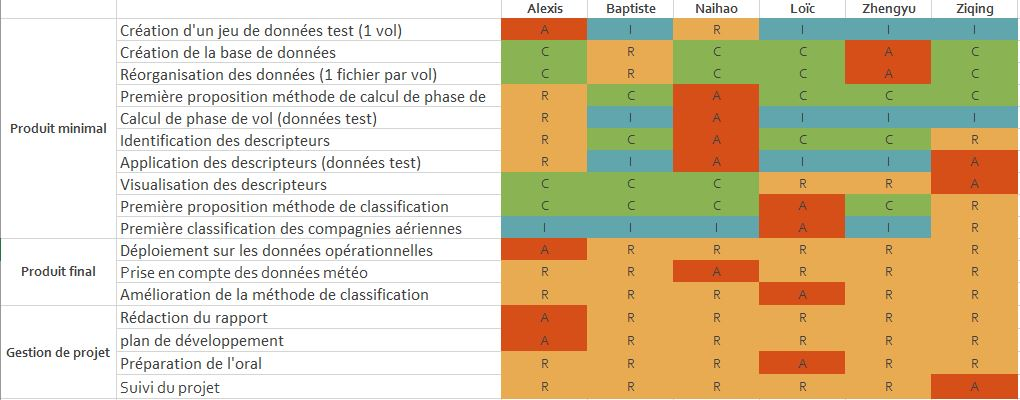
\includegraphics[width=15cm]{RACI}
	\caption{matrice RACI, R:responsible, A:accountable, C:consultable, I:informed}
	\label{fig:raci}
\end{figure}
\section*{Suivi}
\addcontentsline{toc}{section}{Suivi}
Afin que la communication au sein du projet soit de bonne qualité, nous avons mis en place un drive google où sont stockés les documents qui concernent la gestion du projet (cahier charge, compte rendu de réunion,...). Afin d'assurer les travaux de développement et de rédaction de document qui sont souvent fait en équipe, nous avons mis en place un répertoire github. Ces deux répertoires sont accessibles et modifiables depuis n'importe quel poste et par n'importe quel membre du projet. 

Chaque semaine, une réunion sera organisé ce qui permettra de faire un point régulier de l'avancement du projet. Il permettra aussi à chaque membre de poursuivre les tâches qui lui sont attribuées.

D'autre part, nous utiliserons la librairie pandas sous python pour assurer le traitement des données, ainsi que django pour réaliser des applications web. En ce qui concerne la partie gestion de projet, nous utiliserons la suite office ainsi que latex pour rédiger les rendus.

\section*{Organigramme}
\addcontentsline{toc}{section}{Organigramme}
Voici ici l'organigramme correspondant à notre projet.
\begin{figure}[!ht]
	\centering
	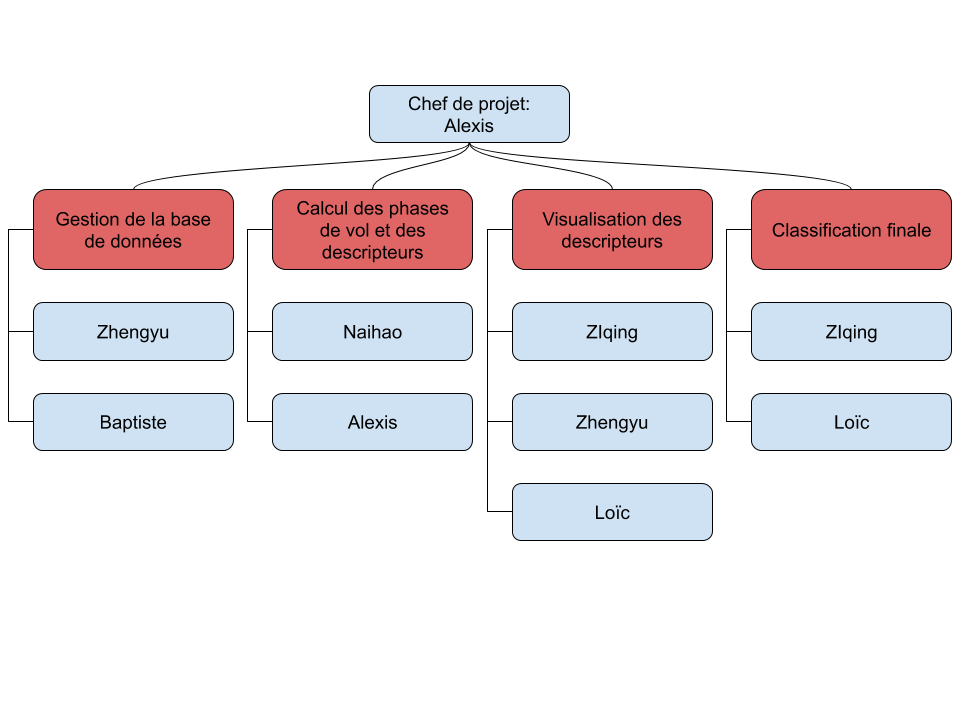
\includegraphics[width=10cm]{Organigramme}
	\caption{Organigramme}
	\label{fig:Organigramme}
\end{figure}


%%% Local Variables: 
%%% mode: latex
%%% TeX-master: "isae-report-template"
%%% End: 
\chapter*{Analyse des risques}
\addcontentsline{toc}{chapter}{Analyse des risques}
\label{sec:risques}
\section*{Gestion des risques}
\addcontentsline{toc}{section}{Gestion des risques}
La gestion des risques est un point clé dans le succès du projet car elle permet d'agir de manière à ce que les risques identifiés arrivent avec la probabilité la plus faible possible. En concertation avec les membres du projet, nous avons identifié les risques suivant:

\begin{itemize}
	\item Perte des données. Une panne matériel peut survenir à tout moment et endommager les données. Ce risque reste assez faible et on peut toujours récupérer les données en les téléchargeant une nouvelle fois.
	
	\item Difficulté d'accès aux données. Si les données sont stockées sur un ordinateur personnel, il y a un risque que cela ralentisse le développement des codes de calculs. C'est pourquoi nous avons envisagé de stocker les données sur un disque accessible depuis n'importe quel ordinateur de l'école.
	
	\item Logiciel inconnu par certain membre du groupe. Nous devrons prendre en compte le fait que tous les membres ne connaissent pas les librairies utilisés et donc évaluer le temps de travail en fonction de cela.
	
	\item Crise du coronavirus. Dans le contexte actuel, il est très probable qu'un des membres tombent malade ou que la communication entre les membres soient plus difficile. Nous devons donc faire en sorte que la majorité des tâches puissent se faire depuis un ordinateur personnel.
	
	\item Mauvaise communication interne. La plupart du travail sera faite en dehors des crénaux prévus pour le PIE. Une mauvaise communication pouvant entrainer retarder le retarder l'exécution du projet, nous allons mettre en place un groupe de conversation messenger ainsi qu'un drive Google où seront déposés les documents relatifs à la gestion du projet.
	
\end{itemize}

\section*{Opportunités}
\addcontentsline{toc}{section}{Opportunités}
%%% Local Variables: 
%%% mode: latex
%%% TeX-master: "isae-report-template"
%%% End: 





\end{document}